% Created 2020-05-12 Tue 13:58
% Intended LaTeX compiler: pdflatex
\documentclass[11pt]{article}
\usepackage[utf8]{inputenc}
\usepackage[T1]{fontenc}
\usepackage{graphicx}
\usepackage{grffile}
\usepackage{longtable}
\usepackage{wrapfig}
\usepackage{rotating}
\usepackage[normalem]{ulem}
\usepackage{amsmath}
\usepackage{textcomp}
\usepackage{amssymb}
\usepackage{capt-of}
\usepackage{hyperref}
\usepackage{minted}
\usepackage{url}
\usepackage{mathtools}
\usepackage{natbib}
\usepackage[dvipsnames]{xcolor}
\usepackage{amsmath}
\DeclareMathOperator*{\argmax}{arg\,max}
\DeclareMathOperator*{\argmin}{arg\,min}
\newcommand{\prob}[0]{\mathrm{p}}
\newcommand{\df}[1]{\mathrm{d} #1}
\newcommand{\samples}[0]{\sim}
\newcommand{\given}[0]{\;|\;}
\newcommand{\xv}[0]{\mathbf{x}}
\newcommand{\Fv}[0]{\mathbf{F}}
\newcommand{\xres}[0]{x_{\mathrm{res}}}
\newcommand{\yres}[0]{y_{\mathrm{res}}}
\newcommand{\dt}[0]{\Delta t}
\newcommand{\av}[0]{\mathbf{a}}
\newcommand{\bv}[0]{\mathbf{b}}
\newcommand{\gv}[0]{\mathbf{g}}
\newcommand{\ov}[0]{\mathbf{o}}
\newcommand{\Ov}[0]{\mathbf{O}}
\newcommand{\scale}[0]{\mathrm{scale}}
\renewcommand*{\tableofcontents}[0]{}
\definecolor{goodgreen}{RGB}{0,140,0}
\author{James Gilles}
\date{12 May 2020}
\title{6.885 Final Project: Inferring Invisible Force Fields using Gaussian Processes}
\hypersetup{
 pdfauthor={James Gilles},
 pdftitle={6.885 Final Project: Inferring Invisible Force Fields using Gaussian Processes},
 pdfkeywords={},
 pdfsubject={},
 pdfcreator={Emacs 26.3 (Org mode 9.3.6)}, 
 pdflang={English}}
\begin{document}

\maketitle
\tableofcontents


\section{Abstract}
\label{sec:org45b522b}
We specify a challenging inference problem involving non-observable force fields affecting particles moving in a 2d plane. We implement and evaluate a baseline solution using Gaussian Processes in Gen \citep{GenPaper}, and outline directions for future work.

Our code is available at: \url{https://github.com/kazimuth/6.885}

\section{Introduction}
\label{sec:orgb8c3784}
There's recently been a surge of interest in using sparsity to accelerate differentiable algorithms, in particular physical simulations. Projects like the Tiramisu compiler \citep{Tiramisu} have successfully leveraged sparsity for large speedups running deep neural networks on GPU. Similarly, the Taichi programming language \citep{Taichi} allows spatially sparse, differentiable physical simulations to be quickly prototyped to run on GPUs.

We believe that tools like these could also be used to accelerate algorithms based on a Bayesian framework. In fact, our initial plan for the project was to attempt to implement Taichi with Gen \citep{GenPaper}, an innovative probabilistic programming environment.

However, we realized that, before beginning porting efforts, it would be useful to have benchmark problems and sample implementations, for the sake of ensuring correctness and comparing performance. So, for this project, we set out to create a small, self-contained benchmark problem using Bayesian inference, which nevertheless exhibits enough complexity to be interesting.

Our benchmark problem involves a set of particles moving on a 2d plane, affected by an externally-imposed static force field. The force field is modeled as a pair of independent Gaussian Processes, one for the x and one for the y component of the field. Given noisy observations of particle positions over a period of time, we use Metropolis-Hastings Monte-Carlo with a custom proposal distribution to infer the values taken by the force field.

\section{Related work}
\label{sec:org937c34a}
Gen \citep{GenPaper} is a probabilistic programming environment integrated with the Julia programming language \citep{Julia}. We implement our baseline solution using a combination of Gen and other Julia libraries.

Our project was inspired by work like Taichi \citep{Taichi} and Tiramisu \citep{Tiramisu}, both of which connect to larger body of work starting with Halide \citep{Halide}. All of these projects involve a separation between the specification of an algorithm and its implementation, allowing the data structures and control flow of the program to be modified while still conforming to a high-level specification.

Our work models a force field using a pair of 2d Gaussian Processes \citep{GPs}. There is a large body of work on methods for sparsely sampling gaussian processes (\cite{UnderstandingSparseGP} \cite{SparseSpectrumGP} \cite{UnifyingGP}). We reviewed some of this literature, but have not yet implemented it in our model.

We had originally intended to use Hamiltonian Monte Carlo \citep{HMC} as part of our inference algorithm, but unfortunately we weren't able to get it working in time.

Our custom proposal distribution requires numerical differentiation of noisy data. We reviewed \cite{NumDiffNonsmooth} for suggestions as to how to reduce noise amplified by differentiation, although we did not use their full algorithm, leaving that for future work.

\section{Problem specification}
\label{sec:orgd895d89}
We select a rectangular region of interest in the real plane, \(R = [x_{\min}, x_{\max}] \times [y_{\min}, y_{\max}] \subset \mathbb{R}^2\), and a span of time \([t_0, t_1] \subset \mathbb{R}\). There are \(n\) particles in the region, moving freely. Each particle has a mass \(m_i\), a position \(\xv_i \in R\) , and a velocity \(\dot{\xv}_i\). A particle's velocity is affected by the force within its grid cell \(\Fv\), and by a drag force which opposes velocity, parameterized by a variable \(k\):
$$\ddot{\xv}_i(t) = \Fv(\xv(t))/m_i - (1-k)\dot{\xv}$$

Particles collide elastically with the boundary of the region, retaining their velocities in the opposite direction. We select initial positions uniformly from the region and set initial velocities to 0:
$$\dot{\xv}_i(t_0) = 0$$
$$\xv_i(t_0) \samples U(R)$$

We model the force as a pair of independent gaussian processes, modeling the x and y components of the force separately. These forces are sampled at an even grid \(\gv\) of points of resolution \(\xres\) by \(\yres\).

The gaussian processes are parameterized by an exponentially decaying covariance kernel with a length scale \(\ell\) and noise parameter \(\sigma\):
\begin{align*}
f(\av, \bv) &= \mathrm{e}^{- \frac{1}{2} \ell \, ||\av-\bv||_2} \\
\Sigma_{ij} &= f(\gv_i, \gv_j) + \begin{cases}
   \sigma & i=j \\
   0 & \mathrm{otherwise}
\end{cases}\\
F_x(\gv_i) &\samples \mathcal{N}(0, \Sigma) \\
F_y(\gv_i) &\samples \mathcal{N}(0, \Sigma) \\
F(\gv_i) &= \begin{bmatrix}
  F_x(\gv_i) \\
  F_y(\gv_i)
\end{bmatrix}
\end{align*}

(where \(||\av||_2\) denotes the \(\ell_2\) norm.)

We place priors on the length scale and noise, using gamma distributions with set parameters:
\begin{align*}
\ell &\samples \Gamma(1, \ell_{\scale}) + \ell_{\min} \\
\sigma &\samples \Gamma(1, \sigma_{\scale}) + \sigma_{\min}
\end{align*}

We discretize time into \(T\) timesteps of length \(\dt\), and approximate positions and velocities using simple Euler integration:
\begin{align*}
\dot{\xv}_i[t+1] &= k (\dot{\xv}_i[t] + \Fv(\xv_i[t]) \dt) \\
\xv_i[t+1] &= \xv_i[t] + \dot{\xv}_i[t] \dt
\end{align*}

The force affecting each particle is chosen by nearest-neighbor sampling from the grid.

\begin{align*}
\Fv(\xv) &= \Fv(\xv_g) \\
\xv_g &= \argmin_{\xv_g \in \gv} ||\xv - \xv_g||_2
\end{align*}

At each time step, we observe particle positions with a noise factor \(o_{\scale}\):
$$\ov_x \samples \mathcal{N}(\xv_x, o_{\scale})$$
$$\ov_y \samples \mathcal{N}(\xv_y, o_{\scale})$$

Note that, once forces and initial positions are chosen, the simulation is deterministic! It is only the observations of particle positions that are noisy.

In this setting, we pose the problem: given a vector of observations \(\Ov\) (and potentially observations of other parameters, such as \(\ell\), \(\sigma\), or ) sample from the posterior distribution \(\prob(\Fv(\gv) \given \Ov)\).

In our implementation, we choose the following values for free parameters:

\begin{center}
\begin{tabular}{lr}
parameter & value\\
\hline
\((x_{min}, x_{max}) \)  & (0.0, 1.0) \\
\((y_{min}, y_{max}) \)  & (0.0, 1.0) \\
\(\xres              \)  &         10 \\
\(\yres              \)  &         10 \\
\(\ell_{\scale}      \)  &        0.1 \\
\(\ell_{\min}        \)  &       0.01 \\
\(\sigma_{\scale}    \)  &        0.1 \\
\(\sigma_{\min}      \)  &       0.01 \\
\(o_{\scale}         \)  &      0.002 \\
\(k\) & 0.9 \\
\(n\) & 10 \\
\end{tabular}
\end{center}

However, these are easy to change.

\section{Implementation \& Results}
\label{sec:orgaf00653}
To start, we implemented and tested a deterministic simulator for the problem, together with static and animated visualizations. Given a force grid and starting positions, our simulator could show us the particle's paths. We show static visualizations here; see the source code to view animated visualizations.

\begin{figure}[htbp]
\centering
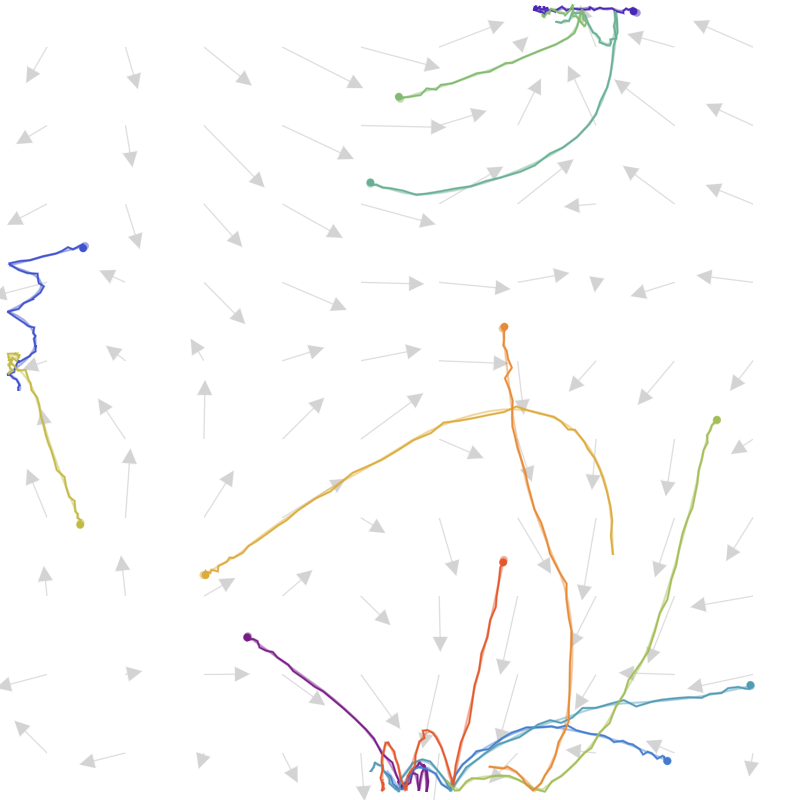
\includegraphics[width=2.5in]{./static.png}
\caption{\label{fig:static}A static visualization of particle paths. Circles represent particle starting points. Gray arrows represent the force grid and are scaled by \(\dt\); that is, they correspond to the amount a particle's velocity will change in one time step. Note the small amount of noise in the observations of the paths. Also note particles bouncing off the boundary.}
\end{figure}

Then, we implemented metropolis-hastings MCMC, with all values observed except for the forces on the grid. This turned out to be barely functional! For more than a few particles, it took an incredibly long time to converge. We realized that this was because it had to guess the entire field essentially a priori. The algorithm was not informed by the observed accelerations applied to the particles. So the vast majority of time, transitions would be rejected, because the particle position traces they generated were too implausible.

We tried accelerating the algorithm by switching to Gen's static modeling language. This gave very good speedups, but didn't address the inefficiency in the algorithm; it was still slow to converge.

Using hamiltonian monte-carlo similarly failed. It's possible this is because gradients were not being propagated well through the body of the our sampling algorithm -- it was somewhat difficult to debug the behavior of gradients.

We realized that we had a lot of information we weren't leveraging in the algorithm. At every time step, we can measure (noisy) changes in a particle's velocity. This should tell us the approximate force value of the grid cell containing the particle. We could use this information by building a custom proposal distribution for the metropolis-hastings transition step, which Gen makes extremely easy.

Of course, measured forces would have some variance; so we would treat them as Gaussians when sampling. Particles might not cross all cells, however. Luckily, we could sample very nice values for unobserved cells using Gaussian Process regression.

We implemented this algorithm\ldots{} and it still didn't work. We tried visualizing the resulting proposals, and noticed that they were \textbf{much noiser} than the original prior, rather than being less noisy! This  turned out to be a result of the differentiation algorithm we were using. Naive second differences turns out to massively magnify noise \citep{NumDiffNonsmooth}. We surveyed denoising algorithms, and decided to smooth the observed accelerations using linear least squares. We fit a cubic function to the x and y components of the observed acceleration traces, and this gave satisfactory results. (See Figure \ref{fig:obsall} for a visualization of this smoothing.)

\begin{figure}[htbp]
\centering
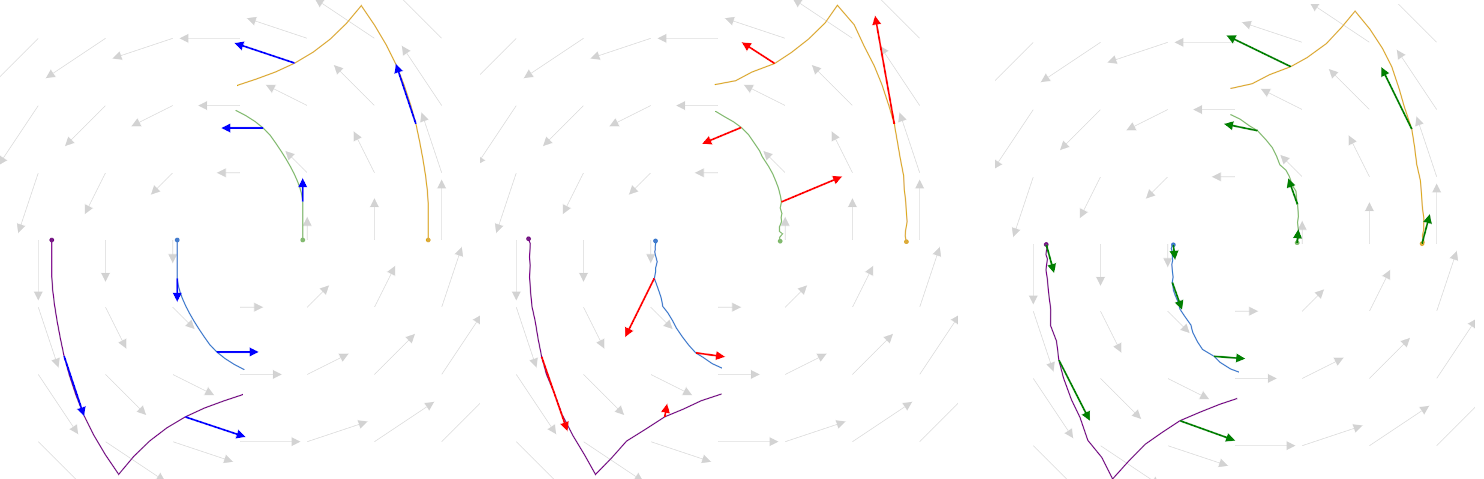
\includegraphics[width=6in]{./obsall.png}
\caption{\label{fig:obsall}Second differences of observed paths. \textcolor{blue}{Blue arrows} show true accelerations at selected timesteps. \textcolor{red}{Red arrows} show accelerations computed from noisy observations using second differences. Note the high variance! \textcolor{goodgreen}{Green arrows} show smoothed second differences. Observe how they are much closer to the true values of the grid cells close to them.}
\end{figure}

This greatly improved convergence times, and allowed us to infer force fields with many particles (20-30).

(One caveat of this algorithm was that it was significantly complicated by boundary behavior. We ended up having to observe whether particles bounced off the boundary without any noise, in order to properly understand the boundaries\ldots{} we leave lifting this restriction to future work.)

We then implemented heirarchical monte carlo, attempting to infer the length scale of the GP kernel and particle initial positions. We were able to get this working by implementing a custom proposal distribution for initial particles, and by moving the length scale proposal into our custom proposal. (Otherwise alternative length scales would never be selected, because they would resample the field without our proposal's knowledge.)

Our algorithm often converges to reasonable approximations of the force field. See Figure \ref{fig:sample} for examples of its outputs.

\begin{figure}[htbp]
\centering
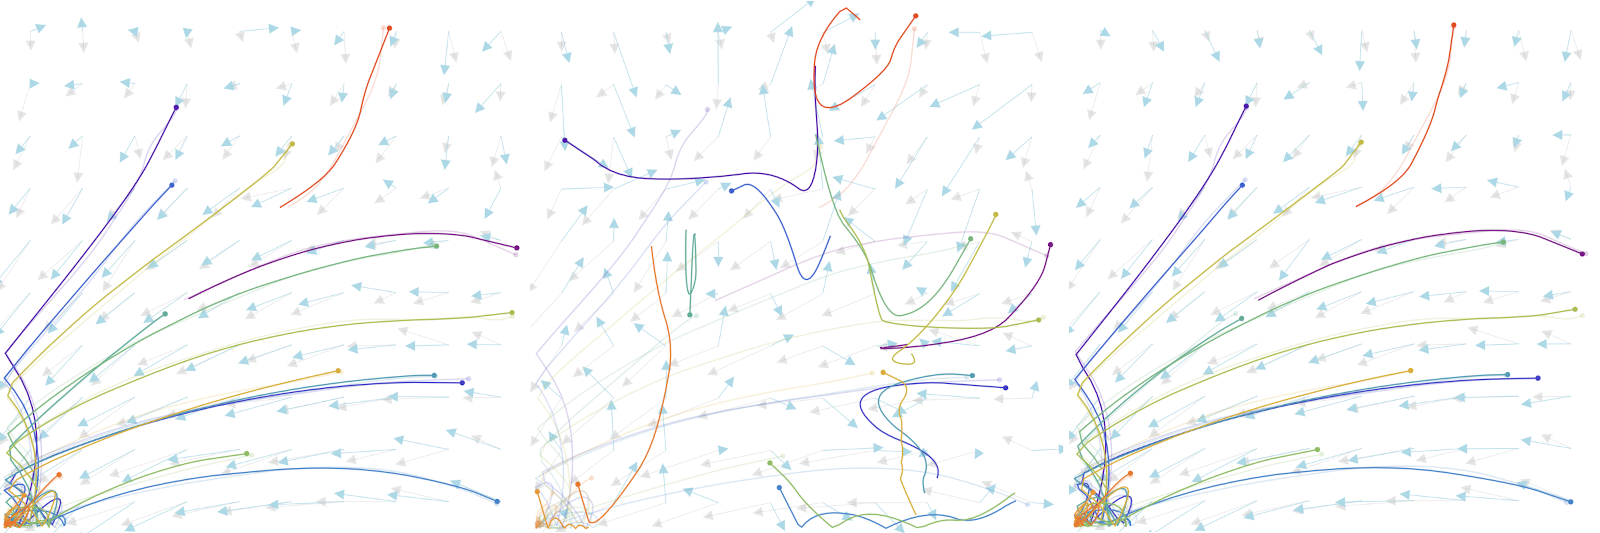
\includegraphics[width=6in]{./result1.png}
\caption{\label{fig:sample}Samples from the posterior distribution after 500 steps of metropolis-hastings. True starting positions and paths are drawn lightly; the inferred force field is drawn lightly, and paths the particles would have taken if placed in it are drawn darkly. Note that the middle case failed to converge in the time limit.}
\end{figure}

\section{Future Work}
\label{sec:org377a189}
In the future, we'd like to try using smarter denoising algorithms, like that proposed in \cite{NumDiffNonsmooth}; or, alternatively, neural denoising.

We'd also like to try implementing a sparse GP approximation, possibly using Taichi, and compare its performance with our implementation.

\bibliography{finalwriteup}
\bibliographystyle{iclr2020conference}
\end{document}